%----------------------------------------------------------------------------------------
%    PACKAGES AND THEMES
%----------------------------------------------------------------------------------------
%\documentclass[aspectratio=169, xcolor=dvipsnames]{beamer} % frames only <--- use this one for your presentation lol
\documentclass[aspectratio=169, xcolor=dvipsnames, handout]{beamer} % for handout
%\documentclass[aspectratio=169, xcolor=dvipsnames, handout, notes]{beamer} % for handout
%\documentclass[aspectratio=169, xcolor=dvipsnames, handout, notes=only]{beamer} % notes only

\setbeameroption{show notes on second screen=right} % remove for presentation

\makeatletter
\def\input@path{{theme/}}
\makeatother
\usetheme{CleanEasy}
\usepackage[utf8]{inputenc}
\usepackage{lmodern}
\usepackage[T1]{fontenc}
% \usepackage[brazil]{babel}
\usepackage{fix-cm}
\usepackage{amsmath}
\usepackage{mathtools}
\usepackage{listings}
\usepackage{xcolor}
\usepackage{hyperref}
\usepackage{graphicx} % Allows including images
\usepackage{booktabs} % Allows the use of \toprule, \midrule and \bottomrule in tables
\usepackage{tikz}
\usetikzlibrary{positioning, shapes, arrows, calc, decorations.pathreplacing, arrows.meta, backgrounds, patterns, overlay-beamer-styles}
\usepackage{etoolbox}
\usepackage{animate}

%----------------------------------------------------------------------------------------
%    LAYOUT CONFIGURATION
%----------------------------------------------------------------------------------------
% Configure code listings
\lstset{
  basicstyle=\ttfamily\small,
  keywordstyle=\color{blue},
  commentstyle=\color{green!60!black},
  stringstyle=\color{red},
  showstringspaces=false,
  breaklines=true,
  frame=single,
  rulecolor=\color{black!30},
  backgroundcolor=\color{black!5},
  numbers=left,
  numberstyle=\tiny\color{black!70},
  numbersep=5pt
}

%----------------------------------------------------------------------------------------
%    TITLE PAGE
%----------------------------------------------------------------------------------------
\title[Natural Language Processing using Transformers]{Natural Language Processing using Transformers}

\author[Kristoffer Brix]{Kristoffer Brix}

\vspace{-2cm}\date{\today}

%----------------------------------------------------------------------------------------


\begin{document}

\begin{frame}[plain]
 \titlepage    
\end{frame} 

\begin{frame}
 \begin{quote}
  Cool article, but everyone already read it, so I will mostly skip it for the presentation and instead show some stuff I made.
  \note[]{
    \begin{itemize}
      \item The article is very hands-on and practical. There are 8 case studies.
      \item There is very little theory -- in two sessions, we will be having more theory on language models, I would like to understand transformer architecture a bit better.
      \item These language models, in essence, are large and very sophisticated neural networks -- I think of them as a function.
      \item I became inspired when I read the article and made some stuff, which I will be presenting today.
      \item Hopefully, by walking through my program, we can get a better feel about how data is transformed and what a simple data pipeline could look like.
    \end{itemize}
    }   
\end{quote}
\hfill -- Kristoffer Brix (about two weeks ago)
\end{frame}

\begin{frame}
 \begin{center}
  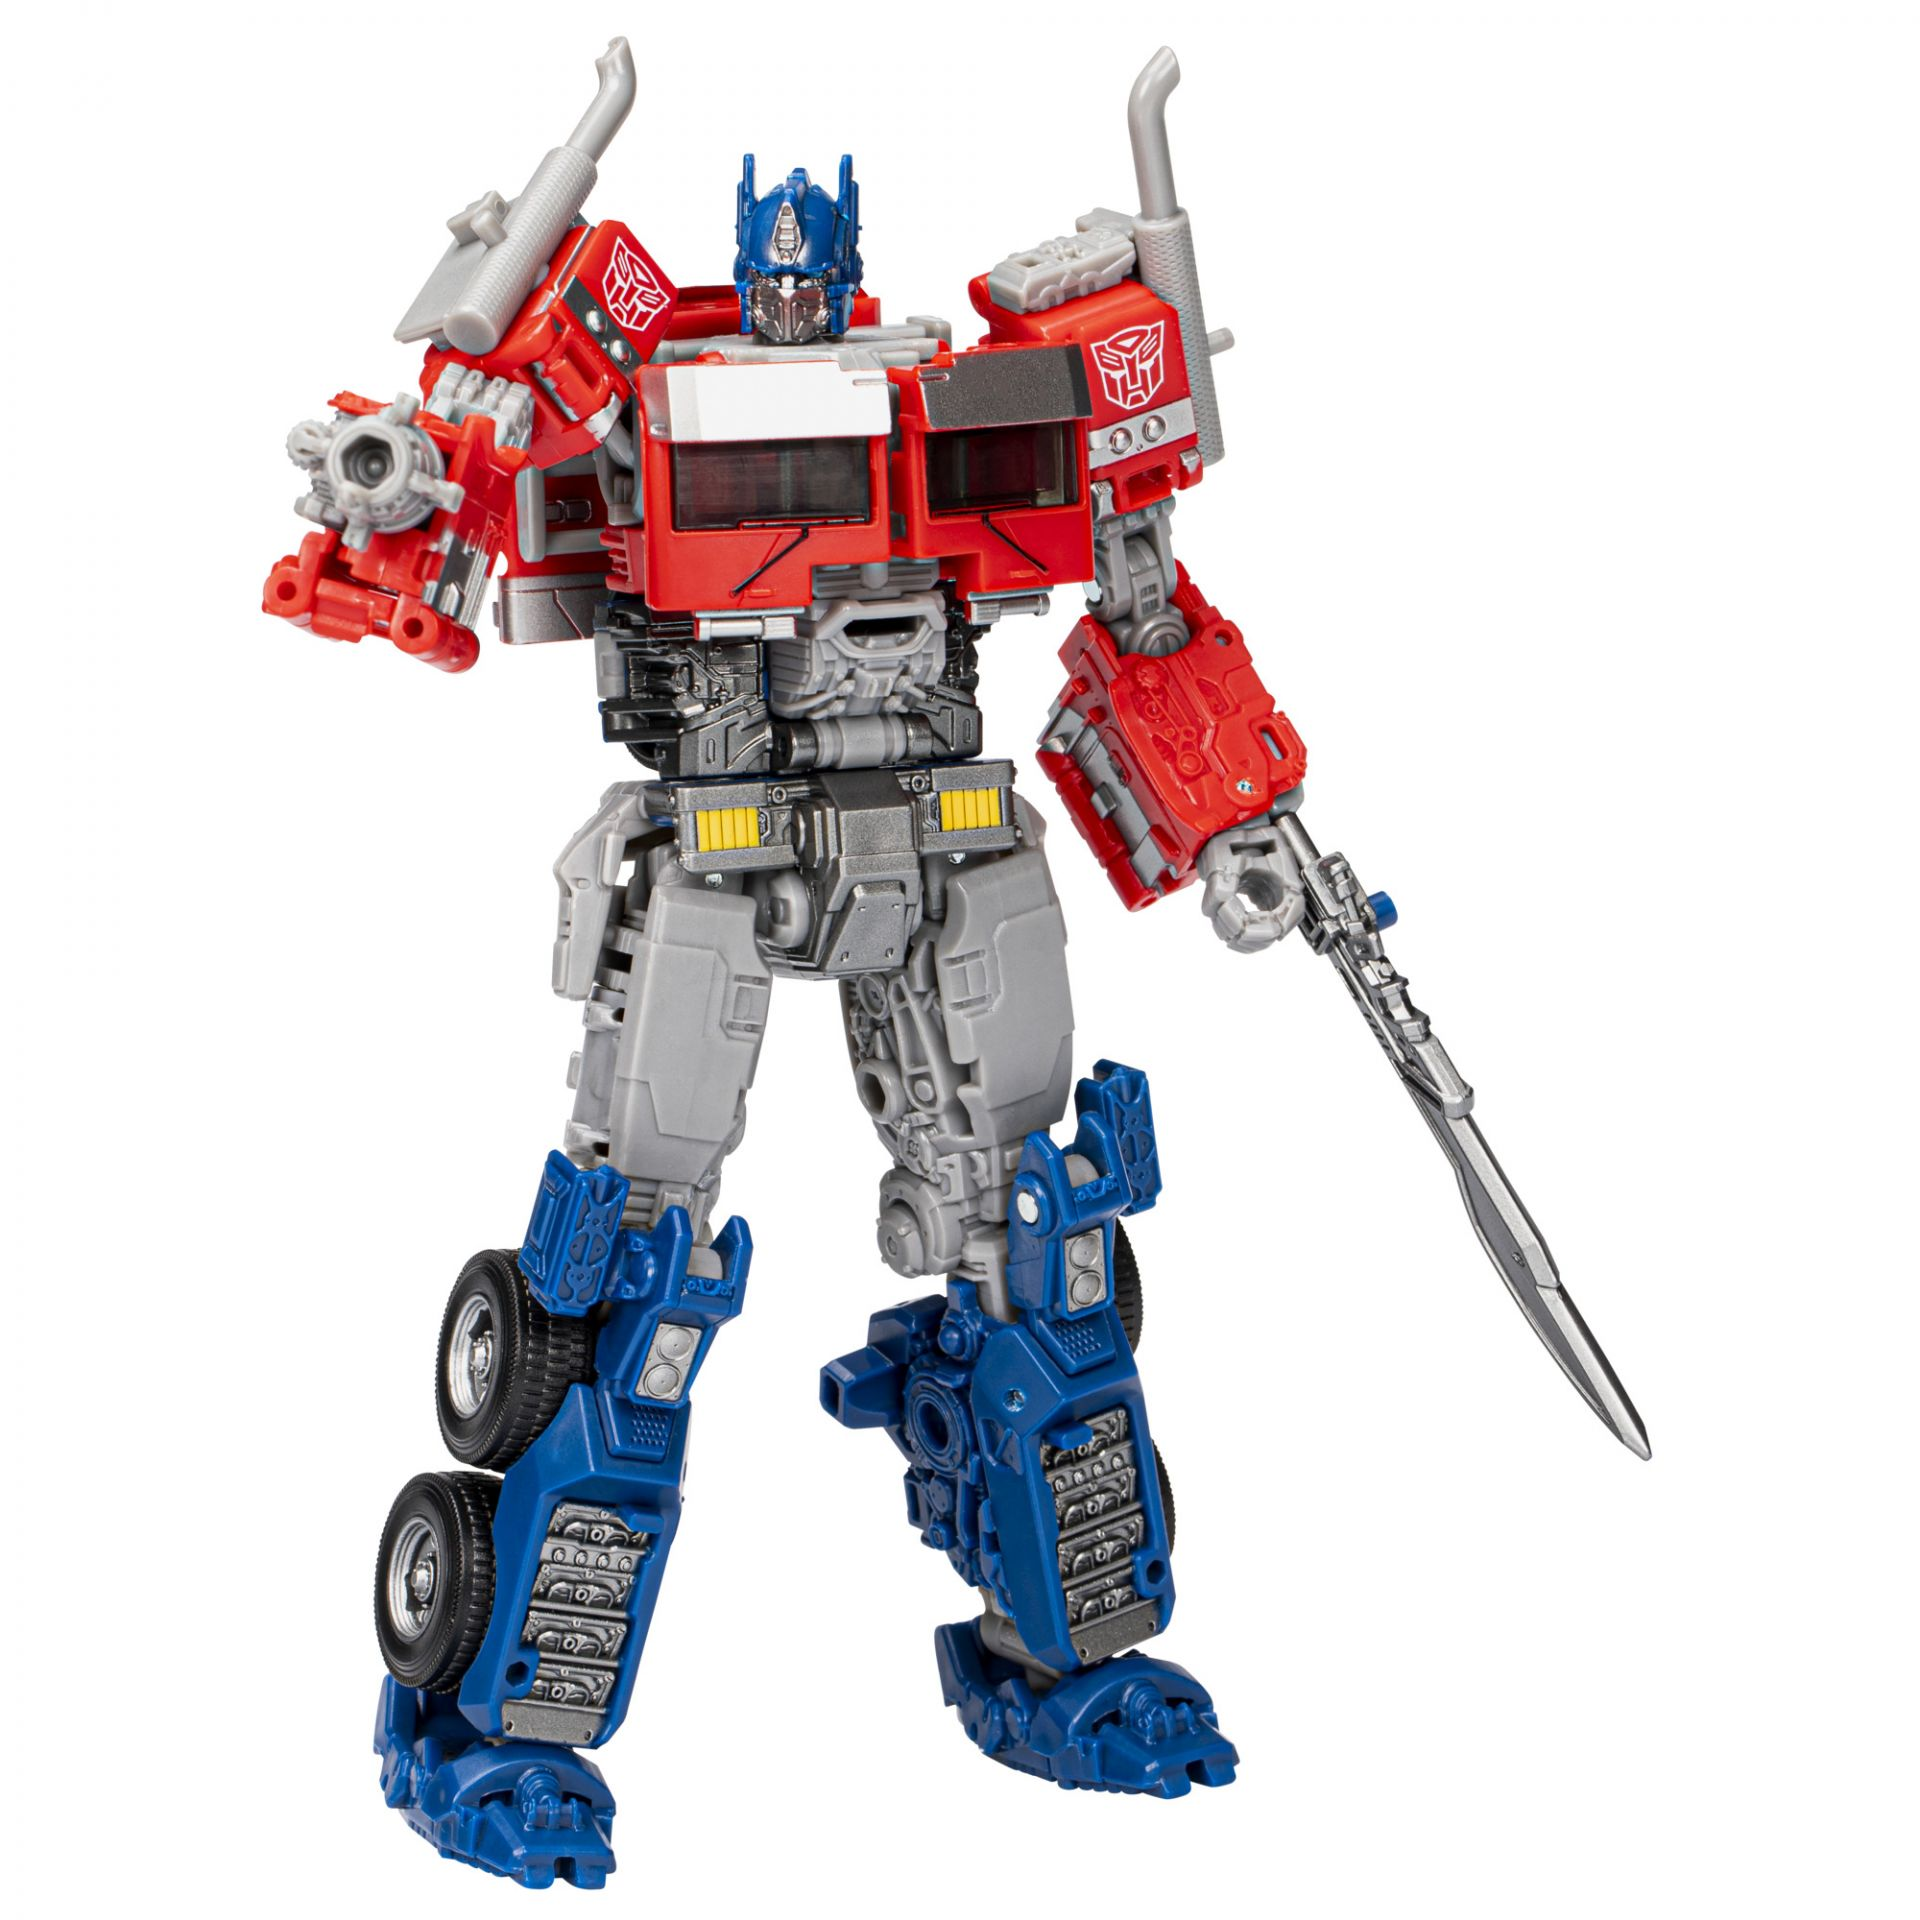
\includegraphics[scale=0.15]{images/optimus-prime.jpg}
 \end{center}
 
  \note[]{
    \begin{itemize}
      \item BERT stands for \textbf{Bidirectional Encoder Representations from Transformers}.
      \item GPT stands for \textbf{Generative Pre-Trained Transformer}.
      \item Optimus Prime is another a Transformer and leader of the Autobots.
    \end{itemize}  
  } 
\end{frame}

\begin{frame}[plain]{Contents}
 \tableofcontents
\end{frame}

\section{What can we download?}  
\begin{frame}{What can we download?}

  On the Hugging Face page for the model.

  \begin{exampleblock}{}
    \begin{center}
     \url{https://huggingface.co/distilbert/distilbert-base-multilingual-cased}
    \end{center}
  \end{exampleblock}
  
  ~\\[-2mm]
  \pause The following files are available for download: \\[2mm]
  
  \begin{itemize}
    \item \textbf{model.onnx} – Cross-platform format for fast inference; compatible with ONNX Runtime, TensorRT. \pause
    \item \textbf{model.safetensors} – Secure, fast-loading PyTorch format; preferred over \texttt{.bin} for safety. \pause
    \item \textbf{pytorch\_model.bin} – Standard PyTorch model; widely used with HuggingFace Transformers. \pause
    \item \textbf{tf\_model.h5} – TensorFlow/Keras-compatible format for training and inference.  
  \end{itemize}

  \note[]{
    \begin{itemize}
      \item Would like to go directly to the source and see what is available. Look at the information about parameter size, downloads per month and some general documentation.
      \item There is also a link the scientific article!
      \item BERT is a family of models with the same base. The other models vary in parameter size and architecture, they have slightly different heads, inputs and outputs.
      \item For example, a) the SQuAD model is used for answering a questions using a given context, b) the SST-2 model for (boolean) sentiment analysis, and c) the GPT model is for generating text by predicting a sequence of tokens.
      \item This is the first trap!
    \end{itemize}
  }
\end{frame}

\section{Architecture}
\begin{frame}{Architecture: Output}
 \begin{center}
  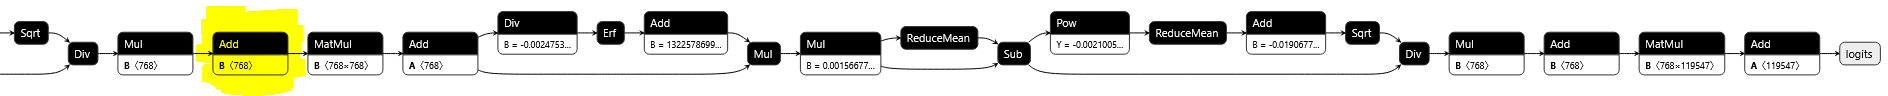
\includegraphics[scale=0.28]{images/model-logits.png}
 \end{center}
 
 \pause
 Notice that the output are \textit{logits} instead of the \textit{last hidden state} (yellow highlight)!
 
 \pause
 ~\\[-2mm]
 119547 is the size of the vocabulary (tokens).
 
 ~\\[-2mm]
 512 is the size of the input sequence.
 
 ~\\[-2mm]
 768 is the size of the last hidden layer.
 
 ~\\[-2mm]
 See also \url{https://netron.app/}.
 
   \note[]{
     \begin{itemize}
       \item The traps has been laid, let us walk into it! Go to \url{https://netron.app/}.
       \item Let us download the model and inspect it.
       \item \texttt{logits} are used to obtain probabilities... but we were supposed to obtain some kind of embedding of the text instead!!
       \item We need to remove this small neural network (this should be understood as a type of classifier) and we will later replace it something else.
       \item The website allows us to inspect various weights in the neural network. When we do Masked Language Modeling, it simply updates the weights to better fit our data using some loss function (cross-entropy loss function).
       \item A simple Python script can convert our model for us, let us look at the script.
     \end{itemize}
   }
\end{frame}

\begin{frame}{Architecture: Input}
 The BERT model requires two input: \pause
 \begin{itemize}
  \item An \texttt{InputIds} object -- an array of integers corresponding to token identifiers in the vocabulary file.\pause 
  \item An \texttt{AttentionMask} object -- an array of boolean values indicating if a token is real or padded (0 = false (padding), 1 = true (real)). \pause
 \end{itemize}

 ~\\[-2mm]
 Just download a tokenizer (lol) -- a sophisticated algorithm for transforming words into tokens, e.g.  [ ``tokenization'' ] $\to$ [ ``token'', ``\#\#ization'' ] (there are many tokenizers and they vary in quality).

   \note[]{
     \begin{itemize}
       \item Let us take a closer look at the input now that we are satisfied with the output -- read off the first line and inspect the vocabulary file, this can also be downloaded from HuggingFace.
       \item Search for the token "hello" and the special token "[MASK]".
       \item Read off the second line. This is very importing for padding later, search for the special token "[PAD]".
       \item Tokenizer are pretty sophisticated algorithms, but are quite common and can be downloaded from anywhere -- watch out for bad quality, look at "BertTokenizers" on GitHub.
     \end{itemize}
   }
\end{frame}

\section{Applying BERT: Demo}
\begin{frame}{Applying BERT (encoder transformer model): Demo}
\pause
 \begin{itemize}
  \item Load in data from the parquet file (free and open-source column-oriented data from Apache, efficient compression and encoding). \pause
  \item Load in a tokenizer and vocabulary file. \pause
  \item Encode text data using the tokenizer to produce an \texttt{InputIds} and \texttt{AttentionMask} object (inputs for BERT). \pause
  \item \textit{Apply} the BERT model (think of it as a function, in essence, BERT is ``just'' a (highly) sophisticated neural network) (it is similar to what we do in \texttt{R} with with the \texttt{stats::predict} function on \texttt{newdata}). \pause
  \item Extract the embedding, e.g. the first embedding or the mean embedding. \pause
  \item Pipe the embedding into a new model.
 \end{itemize}

   \note[]{
     \begin{itemize}
       \item Time for the first demo, read up the steps and then go into the C\# code, then look at the two \texttt R scripts.
     \end{itemize}
   }
\end{frame}

\section{Applying GPT: Demo}
\begin{frame}{Applying GPT (decoder transformer model): Demo}
\pause
 \begin{itemize}
  \item Load in data from the parquet file (like before). \pause
  \item Load in ``large language model'' (e.g. \href{https://lmstudio.ai/}{\underline{LM Studio}}, \href{https://ollama.com/}{\underline{Ollama}}, the cloud, etc.). \pause
  \item Build an API to communicate with large language model service (see \url{https://platform.openai.com/docs/api-reference/chat/create}). \pause
  \item Create a prompt where the next predicted token will be the class label (hopefully) -- this is ``classification as generation''.
 \end{itemize}

   \note[]{
     \begin{itemize}
       \item Time for the second demo, read up the steps, go to the two links, execute something in \texttt{bash} then go into the C\# code. Note that \texttt{bash} is not installed on Windows by default, it is a Linux thing. \texttt{curl} is installed on Windows, but I can never seem to get it to work, maybe the syntax is wrong.
     \end{itemize}
   }
\end{frame}

\section{Additional Links}
\begin{frame}{Additional Links}
\pause
 \begin{itemize}
  \item  ONNX Get Started Documentation: \url{https://onnxruntime.ai/docs/get-started}. \pause
  \item ONNX Tutorials: \url{https://github.com/onnx/tutorials}. \pause
  \item ModernBert \url{https://huggingface.co/blog/modernbert}. \pause
  \item \texttt{llama.cpp}: \url{https://github.com/ggml-org/llama.cpp}. \pause
  \item Shopping (run e.g. Llama 3.3 70B model at 8-10 t/s): \url{https://frame.work/dk/en/products/desktop-diy-amd-aimax300/configuration/new}.
 \end{itemize}

   \note[]{
     \begin{itemize}
       \item Conceptually, we are using the two types of models very differently, even though they fall into the family of transformers.
       \item We use BERT to extract covariates and use these covariates for classification (statistical modeling).
       \item We use GPT for to predict the next token, where the next token happens to be some class -- this goes well because the model is VERY big.
     \end{itemize}
   }
\end{frame}

\end{document}
